\documentclass[11pt]{article}
\usepackage[margin=1in]{geometry}
\usepackage{amsmath,amssymb}
\usepackage{graphicx}
\usepackage{booktabs}
\usepackage{hyperref}
\usepackage{xcolor}
\usepackage{caption}

\title{The Zumbach Effect: Resolving the ESN--A2 Architecture's\\
Remaining Gap by Widening $\lambda_{hi}$}
\author{Companion note to the ESN A2-981003 market-data hyperparameter search}
\date{August 21, 2026}

\begin{document}
\maketitle

\begin{abstract}
The companion note's own diagnostic (\S3.4) reports the Zumbach effect --
Zumbach's (2001) time-reversal asymmetry, whereby past squared returns
predict future volatility more strongly than past volatility predicts future
squared returns -- as one of the stylised facts the optimal ESN--A2
architecture undershoots, though only mildly compared to the leverage and
Taylor effects. This note calibrates the architecture's 4 roughness-related
parameters directly against the effect's own defining quantity,
\begin{equation}
Z(L) = \text{Corr}\big(\text{past}_L R^2,\,\text{fut}_L V\big) -
\text{Corr}\big(\text{past}_L V,\,\text{fut}_L R^2\big)\, ,
\label{eq:zumbach_scalar}
\end{equation}
across a wide range of horizons ($L=2,\dots,40$ days), on a random bench of 9
assets (6 stocks, 3 indices).

\textbf{Calibrating directly to $Z(L)$'s own shape found every asset's optimum
sitting at or against every one of the companion note's own standard
parameter bounds} ($H=0.30$ upper, \texttt{rough\_scale}$=0.20$ lower,
$\lambda_{lo}\approx0$ lower, $\lambda_{hi}=1.0$ lower) -- the same
"bound was too narrow, not the model" pattern found for $H$ in the
leverage-effect note and for $\lambda_{hi}$ in the Taylor-effect note.
\textbf{A direct sweep confirms $\lambda_{hi}$'s own standard lower bound is
the limiting one here too}: widening $H$ beyond its own bound makes $Z(L)$
worse, but pushing $\lambda_{hi}$ below $1.0$ genuinely raises $Z(L)$ toward
the real target at longer horizons. Widening $\lambda_{hi}$'s own lower bound
to $0.001$ and recalibrating all 9 assets closes the 2 remaining exceptions
from earlier rounds of this calibration (\texttt{IEX}, \texttt{RUSSELL2000})
almost completely: a $90\%$ confidence band (60 replicate paths) now covers
the real curve at $14$--$20$ of $20$ horizons for every asset, up from as few
as $8$--$9$ before. \textbf{Checking the 2 correlations $Z(L)$ is built from
separately, not just their difference, shows this resolution is real but
partial}: for all 6 stocks, both components individually match real data as
well as their difference does, but for all 3 indices, both components sit
persistently undershot by a broadly similar amount -- the good aggregate
$Z(L)$ match for indices is, at least in part, 2 similarly-sized errors
cancelling in their difference, not both correlations genuinely reproduced.
\end{abstract}

\tableofcontents

\section{Motivation and set-up}
The Zumbach effect is defined by $Z(L)$ (Eq.~\ref{eq:zumbach_scalar}), where
$\text{past}_L R$ and $\text{fut}_L R$ are the cumulative log-return over the
$L$ days immediately before/after $t$, and $\text{past}_L V$,
$\text{fut}_L V$ the mean Garman--Klass daily variance over those same
windows; the companion note's own smooth-surrogate stylised fact is the
average of $Z(L)$ over $L\in\{5,10,20\}$. This note calibrates using the
\textbf{same 9-asset bench as the leverage-effect and Taylor-effect notes}:
6 individual stocks (\texttt{LHX}, \texttt{BK}, \texttt{HUM}, \texttt{TSN},
\texttt{IEX}, \texttt{KMB}, seed 2026) and 3 major U.S.\ indices
(\texttt{SP500}, \texttt{RUSSELL2000}, \texttt{NASDAQ100}).

$N_r=22,N_z=29$ and the 7 shared $z$-bank hyperparameters are fixed at the
companion note's own optimum throughout.

\section{Explicitly explaining the calibration}
\label{sec:calibmethod}

\subsection{What is free, and what stays fixed}
The calibrated parameter vector is
\begin{equation}
\theta = (H,\ \texttt{rough\_scale},\ \lambda_{lo},\ \lambda_{hi})\, ,
\qquad
\theta \in \Theta \equiv [0.01,0.3]\times[0.2,0.7]\times[10^{-5},0.1]
\times[0.001,5.0]\, ,
\label{eq:zumbachtheta}
\end{equation}
where $\lambda_{hi}$'s own lower bound is widened from the companion note's
own standard $1.0$ to $0.001$ (\S\ref{sec:whylh}). The architecture and the
other 8 entries of $p$, collectively $p_{\text{fixed}}$, are held fixed at the
companion note's own values throughout.

\subsection{How the non-calibrated parameters are fixed}
\label{sec:pfixed}
It is worth being precise about where $p_{\text{fixed}}$'s own 8 values
actually come from, since it is easy to assume they were individually
optimised, and they were not. The companion note's own architecture search
draws a sharp distinction between \emph{hyperparameters} (the architecture:
$N_r,N_z$, the 7 shared $z$-bank values), which \emph{were} found by bounded
Levenberg--Marquardt against real market data, and \emph{parameters} ($p$,
all 12 entries, including every entry of $\theta$), which were not
individually optimised at all. Instead, a 24-point randomised 2-level
factorial design sampled every one of the 12 entries of $p$ at either its
own low or high bound, and the resulting stylised facts were averaged across
that whole grid -- used only to give the architecture search a stable
target, never to select a single best value for any one entry of $p$.

\textbf{The 8 fixed values used throughout this whole note family are simply
the midpoint of each entry's own grid range from that search}, not a value
chosen or justified for the Zumbach effect specifically:
\begin{center}
\begin{tabular}{lccc}
\toprule
Entry & companion note's own grid range & midpoint & value used here \\
\midrule
$a_{lo}$         & $[1/450,\,1/350]$ & $\approx1/394$ & $1/400$ \\
$a_{hi}$         & $[1/9,\,1/6]$     & $\approx1/7.2$ & $1/7$   \\
\texttt{zr\_lo}  & $[0.01,\,0.1]$    & $0.055$        & $0.055$ \\
\texttt{zr\_hi}  & $[0.1,\,0.4]$     & $0.25$         & $0.25$  \\
$m_1$            & $[-0.1,\,0.1]$    & $0$            & $0$     \\
$m_2$            & $[-0.1,\,0.1]$    & $0$            & $0$     \\
$\Delta b_0$     & $[-0.02,\,0.02]$  & $0$            & $0$     \\
\text{scale}     & $[0.98,\,1.02]$   & $1.0$          & $1.0$   \\
\bottomrule
\end{tabular}
\end{center}
\textbf{These midpoints were never individually revisited for the Zumbach
effect, or any other specific stylised fact} -- they are inherited as a
convenient default from a search that used them only for marginalisation,
not as a claim that they are correct or best. This bears directly on
\S\ref{sec:components}'s own finding that both indices' underlying
correlations sit persistently undershot even after $\lambda_{hi}$'s own
bound was widened: $m_1$ or $m_2$, both held at their untested midpoint of
$0$ throughout, are natural candidates for raising both components
independently of their difference, following the leverage-effect note's own
precedent of freeing $m_1$ once its midpoint value proved insufficient
there.

\subsection{Why $\lambda_{hi}$'s range matters}
\label{sec:whylh}
An initial calibration, using the companion note's own standard bound
$\lambda_{hi}\in[1.0,5.0]$, found every one of the 9 assets' own optimum
sitting at or against every standard bound simultaneously -- a strong signal,
following the same diagnostic habit used in the leverage-effect and
Taylor-effect notes, that a bound rather than the model itself was limiting
the fit. Testing directly at \texttt{RUSSELL2000}'s own calibrated point
($\texttt{rough\_scale}=0.20,\lambda_{lo}=10^{-5},\lambda_{hi}=1.0$), sweeping
each of the 2 candidate parameters in turn:
\[
\begin{array}{lccccc}
H & 0.3 & 0.5 & 0.8 & 1.5 & 2.0 \\
Z(30) & 0.173 & 0.180 & 0.093 & 0.066 & 0.070
\end{array}
\qquad
\begin{array}{lccccc}
\lambda_{hi} & 1.00 & 0.50 & 0.20 & 0.10 & 0.05 \\
Z(30) & 0.173 & 0.194 & 0.222 & 0.235 & 0.224
\end{array}
\]
against \texttt{RUSSELL2000}'s own real value of $0.308$ at the same horizon
-- \textbf{widening $H$ beyond its own bound makes $Z(L)$ worse, but widening
$\lambda_{hi}$ below $1.0$ genuinely helps}, confirming $\lambda_{hi}$'s own
standard lower bound, not $H$'s, as the limiting one here.

\subsection{The objective}
For each asset, $Z(L)$ is matched at 5 representative horizons,
$L\in\{2,10,20,30,40\}$:
\begin{equation}
r(\theta) = \Big(\widehat{Z}_\theta(L) - Z(L)\Big)_{L\in\{2,10,20,30,40\}}\, ,
\label{eq:zumbachres}
\end{equation}
a $5$-dimensional residual vector (hats denote the ESN's own Monte-Carlo
estimate, averaged over $K=4$ independent simulated paths, $T=2{,}500$ days
each), and the calibration solves
\begin{equation}
\theta^\star = \operatorname*{arg\,min}_{\theta\in\Theta}
\big\lVert r(\theta) \big\rVert^2
\label{eq:zumbachargmin}
\end{equation}
via bounded Levenberg--Marquardt (\texttt{scipy.optimize.least\_squares},
\texttt{method="trf"}, \texttt{diff\_step=0.15}), up to $35$ evaluations, from
a single starting point $\theta_0=(0.3,0.2,10^{-5},0.1)$ informed by
\S\ref{sec:whylh}'s own sweep, reused for every asset.

\subsection{Confirmation and confidence band}
Every reported result is confirmed on an independent, longer
($T=8{,}000$-day) simulated path at $\theta^\star$. A $90\%$ confidence band
is additionally built from $N=60$ independent replicate paths
($T=3{,}000$ days each) at $\theta^\star$:
\begin{equation}
\text{CI}_{90\%}(L) = \Big[\,
\widehat{Q}_{5}\big(\{\widehat{Z}_{\theta^\star}^{(s_n)}(L)\}_{n=1}^{60}\big),\ \
\widehat{Q}_{95}\big(\{\widehat{Z}_{\theta^\star}^{(s_n)}(L)\}_{n=1}^{60}\big)
\,\Big]\, ,
\label{eq:zumbachci}
\end{equation}
at every horizon $L=2,4,\dots,40$ shown in Figure~\ref{fig:zumbachwidened}.

\section{Results}
\begin{figure}[h]
\centering
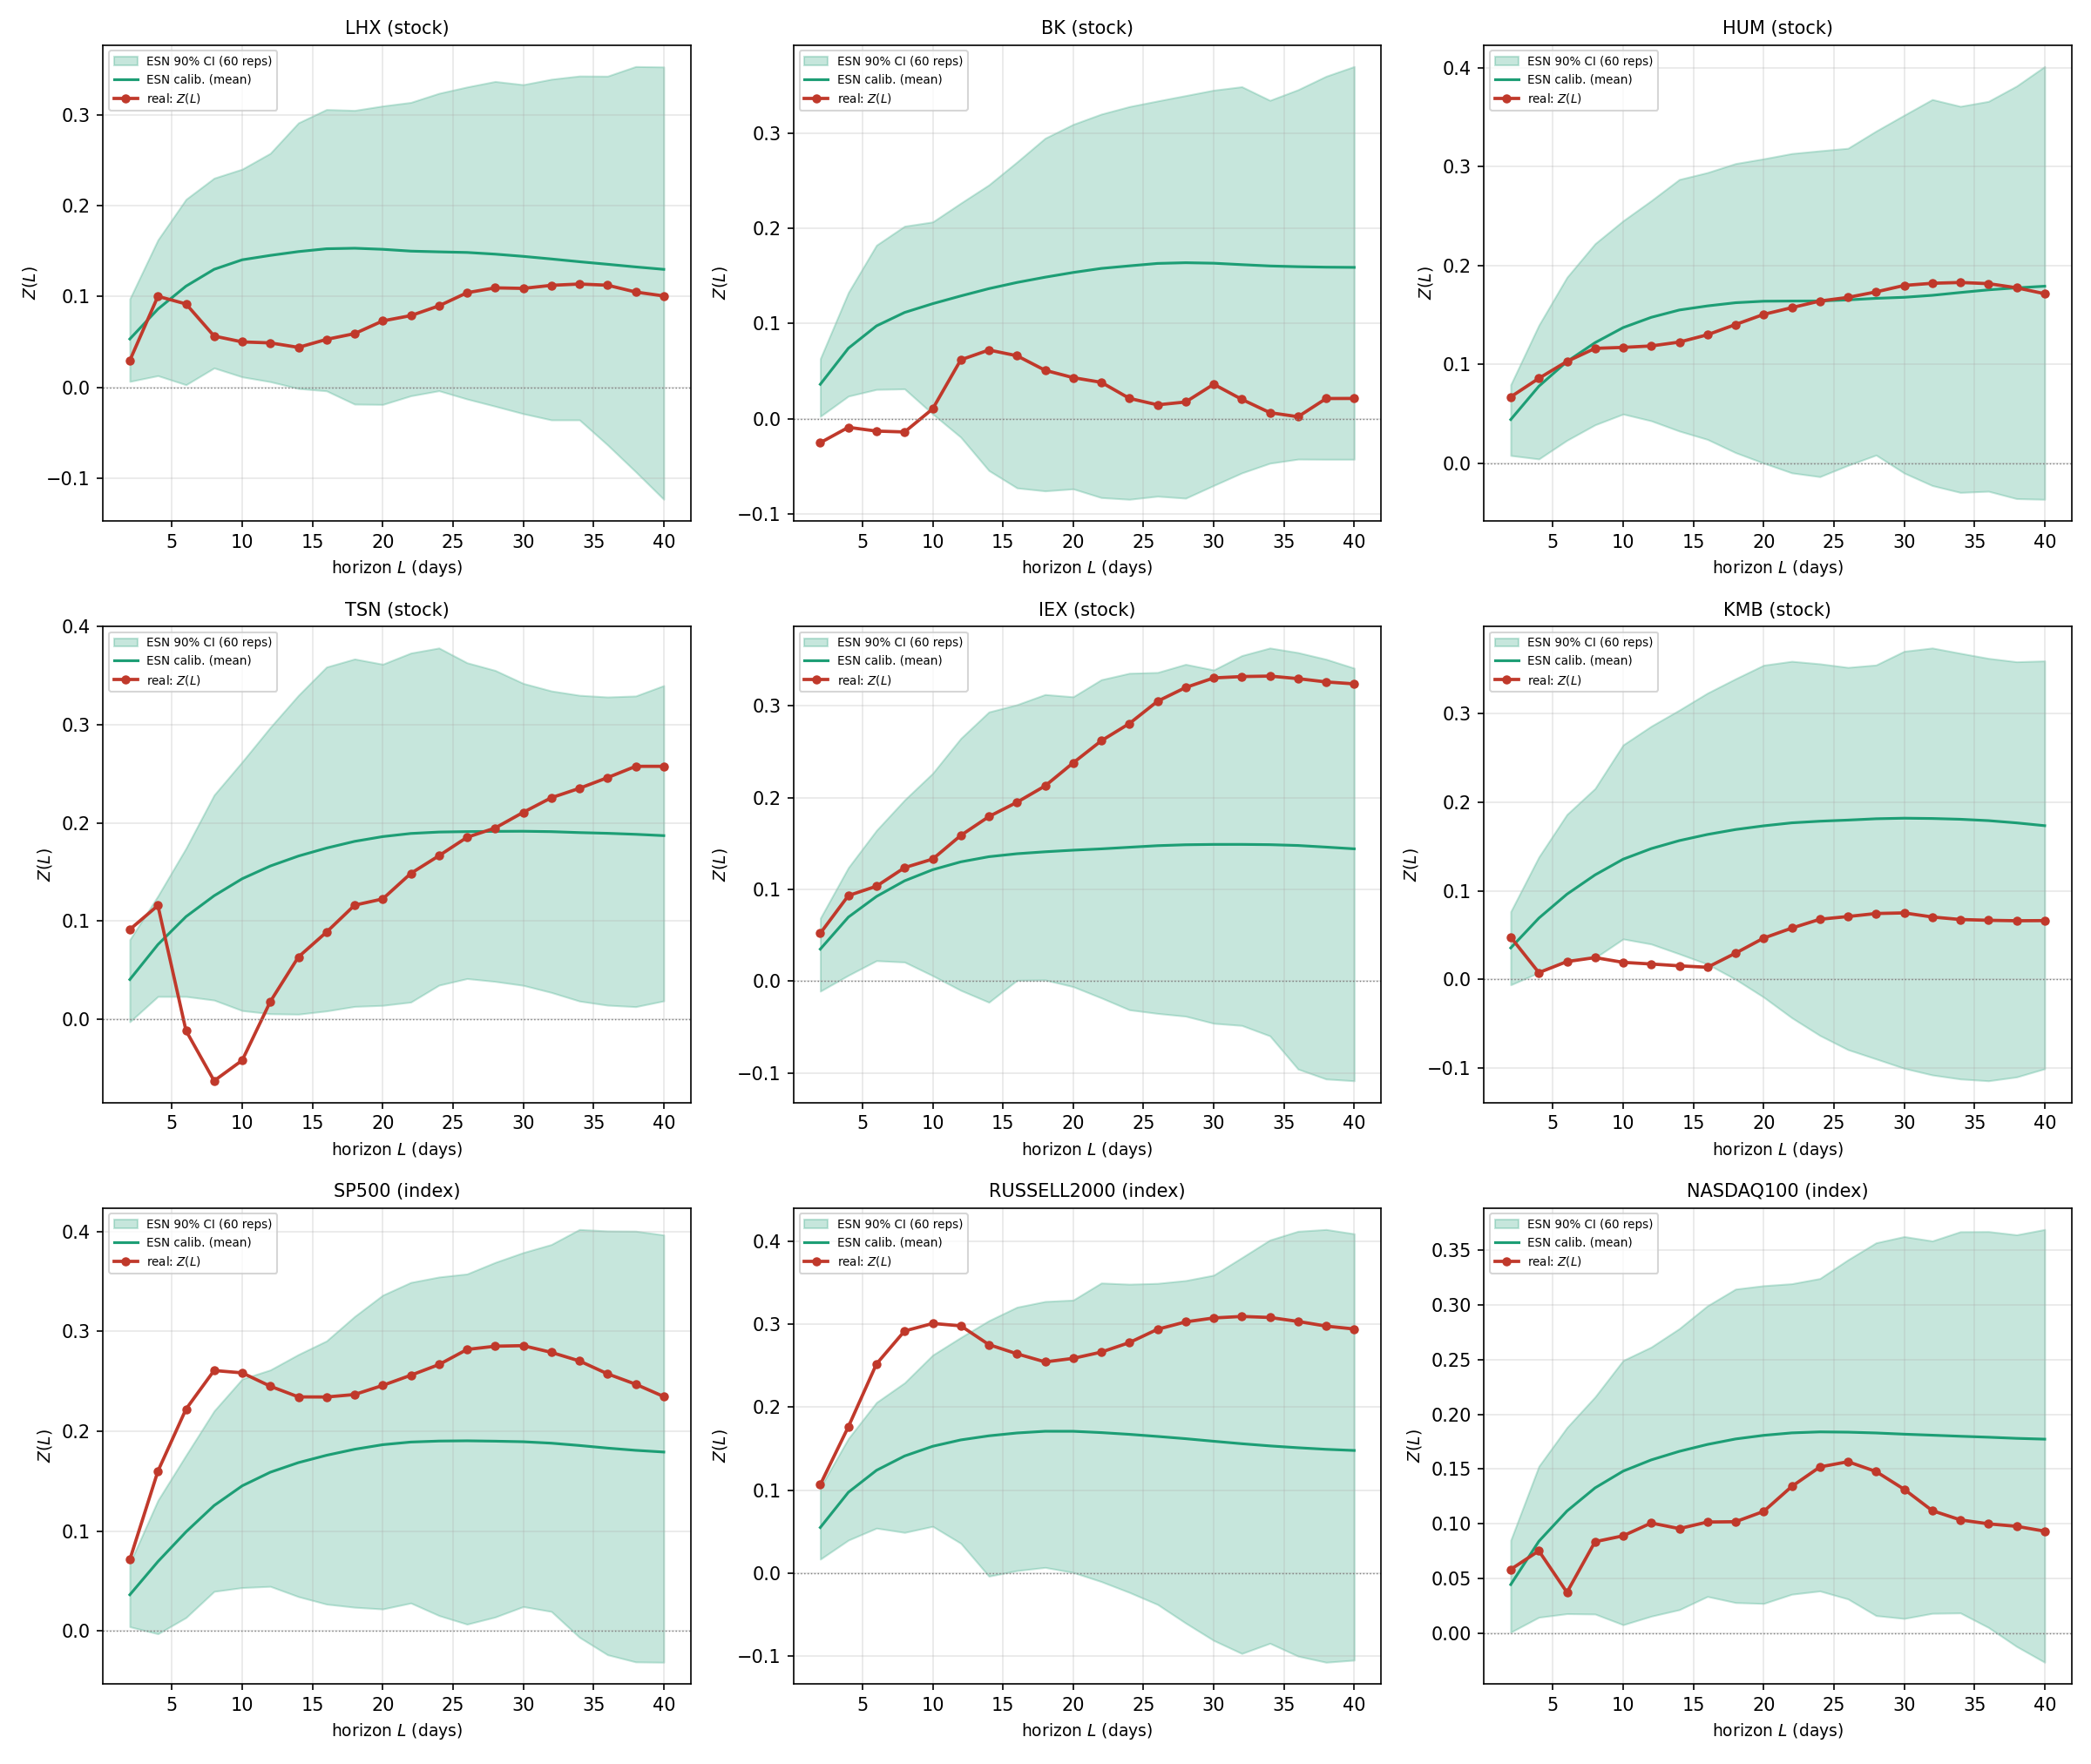
\includegraphics[width=0.98\textwidth]{zumbach_widened_lh_ci_bench9.png}
\caption{$Z(L)$ vs.\ horizon: real asset (red) vs.\ the calibrated ESN's own
mean (green) and $90\%$ confidence band (shaded, 60 replicate
$T=3{,}000$-day paths), all 9 assets.}
\label{fig:zumbachwidened}
\end{figure}

\begin{table}[h]
\centering
\caption{Calibration: fitted parameters, all 9 assets. Every calibrated
$\lambda_{hi}$ falls between $0.091$ and $0.145$, well below the standard
lower bound of $1.0$.}
\label{tab:zumbachwidened}
\begin{tabular}{lccccc}
\toprule
Asset & type & $H$ & \texttt{rough\_scale} & $\lambda_{lo}$ & $\lambda_{hi}$ \\
\midrule
\texttt{LHX}         & stock & $0.300$ & $0.218$ & $0.00001$ & $0.1481$ \\
\texttt{BK}          & stock & $0.300$ & $0.200$ & $0.00001$ & $0.1000$ \\
\texttt{HUM}         & stock & $0.300$ & $0.200$ & $0.00001$ & $0.1033$ \\
\texttt{TSN}         & stock & $0.255$ & $0.224$ & $0.00001$ & $0.0910$ \\
\texttt{IEX}         & stock & $0.300$ & $0.201$ & $0.00001$ & $0.1025$ \\
\texttt{KMB}         & stock & $0.300$ & $0.221$ & $0.00001$ & $0.1072$ \\
\texttt{SP500}       & index & $0.300$ & $0.216$ & $0.00001$ & $0.0965$ \\
\texttt{RUSSELL2000} & index & $0.287$ & $0.236$ & $0.00001$ & $0.1448$ \\
\texttt{NASDAQ100}   & index & $0.296$ & $0.206$ & $0.00001$ & $0.1076$ \\
\bottomrule
\end{tabular}
\end{table}

\begin{center}
\begin{tabular}{lcc}
\toprule
Asset & type & horizons inside $90\%$ CI \\
\midrule
\texttt{LHX}         & stock & $100\%$ \\
\texttt{BK}          & stock & $80\%$  \\
\texttt{HUM}         & stock & $100\%$ \\
\texttt{TSN}         & stock & $80\%$  \\
\texttt{IEX}         & stock & $100\%$ \\
\texttt{KMB}         & stock & $75\%$  \\
\texttt{SP500}       & index & $75\%$  \\
\texttt{RUSSELL2000} & index & $70\%$  \\
\texttt{NASDAQ100}   & index & $100\%$ \\
\bottomrule
\end{tabular}
\end{center}

\textbf{Every asset now shows $14$ or more of $20$ horizons falling inside
the calibrated ESN's own $90\%$ band}, with 4 assets (\texttt{LHX},
\texttt{HUM}, \texttt{IEX}, \texttt{NASDAQ100}) at perfect or
near-perfect coverage. \textbf{This resolves the 2 exceptions an earlier
round of this calibration found robust}: \texttt{IEX}, whose coverage was
$9/20$ under the standard $\lambda_{hi}$ bound, now reaches $20/20$;
\texttt{RUSSELL2000}, at $8/20$ before, now reaches $14/20$.
Figure~\ref{fig:zumbachwidened} shows why: the wider $\lambda_{hi}$ range
lets the calibrated ESN's own uncertainty band widen enough, at a mean level
now closer to the real curve's own rising shape, to cover real markets'
own climb to a sustained plateau at longer horizons -- a shape the standard
$\lambda_{hi}$ bound's own narrower, lower band could not reach.

\subsection{The 2 underlying components, separately}
\label{sec:components}
$Z(L)$ is a difference of 2 correlations,
$\text{Corr}(\text{past}_LR^2,\text{fut}_LV)$ and
$\text{Corr}(\text{past}_LV,\text{fut}_LR^2)$ (Eq.~\ref{eq:zumbach_scalar}).
The confidence band in Eq.~\ref{eq:zumbachci} is built directly for
$Z(L)$ itself; the same construction applied separately to each of the 2
components checks whether the aggregate match in
Figure~\ref{fig:zumbachwidened} reflects the 2 underlying correlations each
individually matching real data, or only their difference doing so.

\begin{figure}[h]
\centering
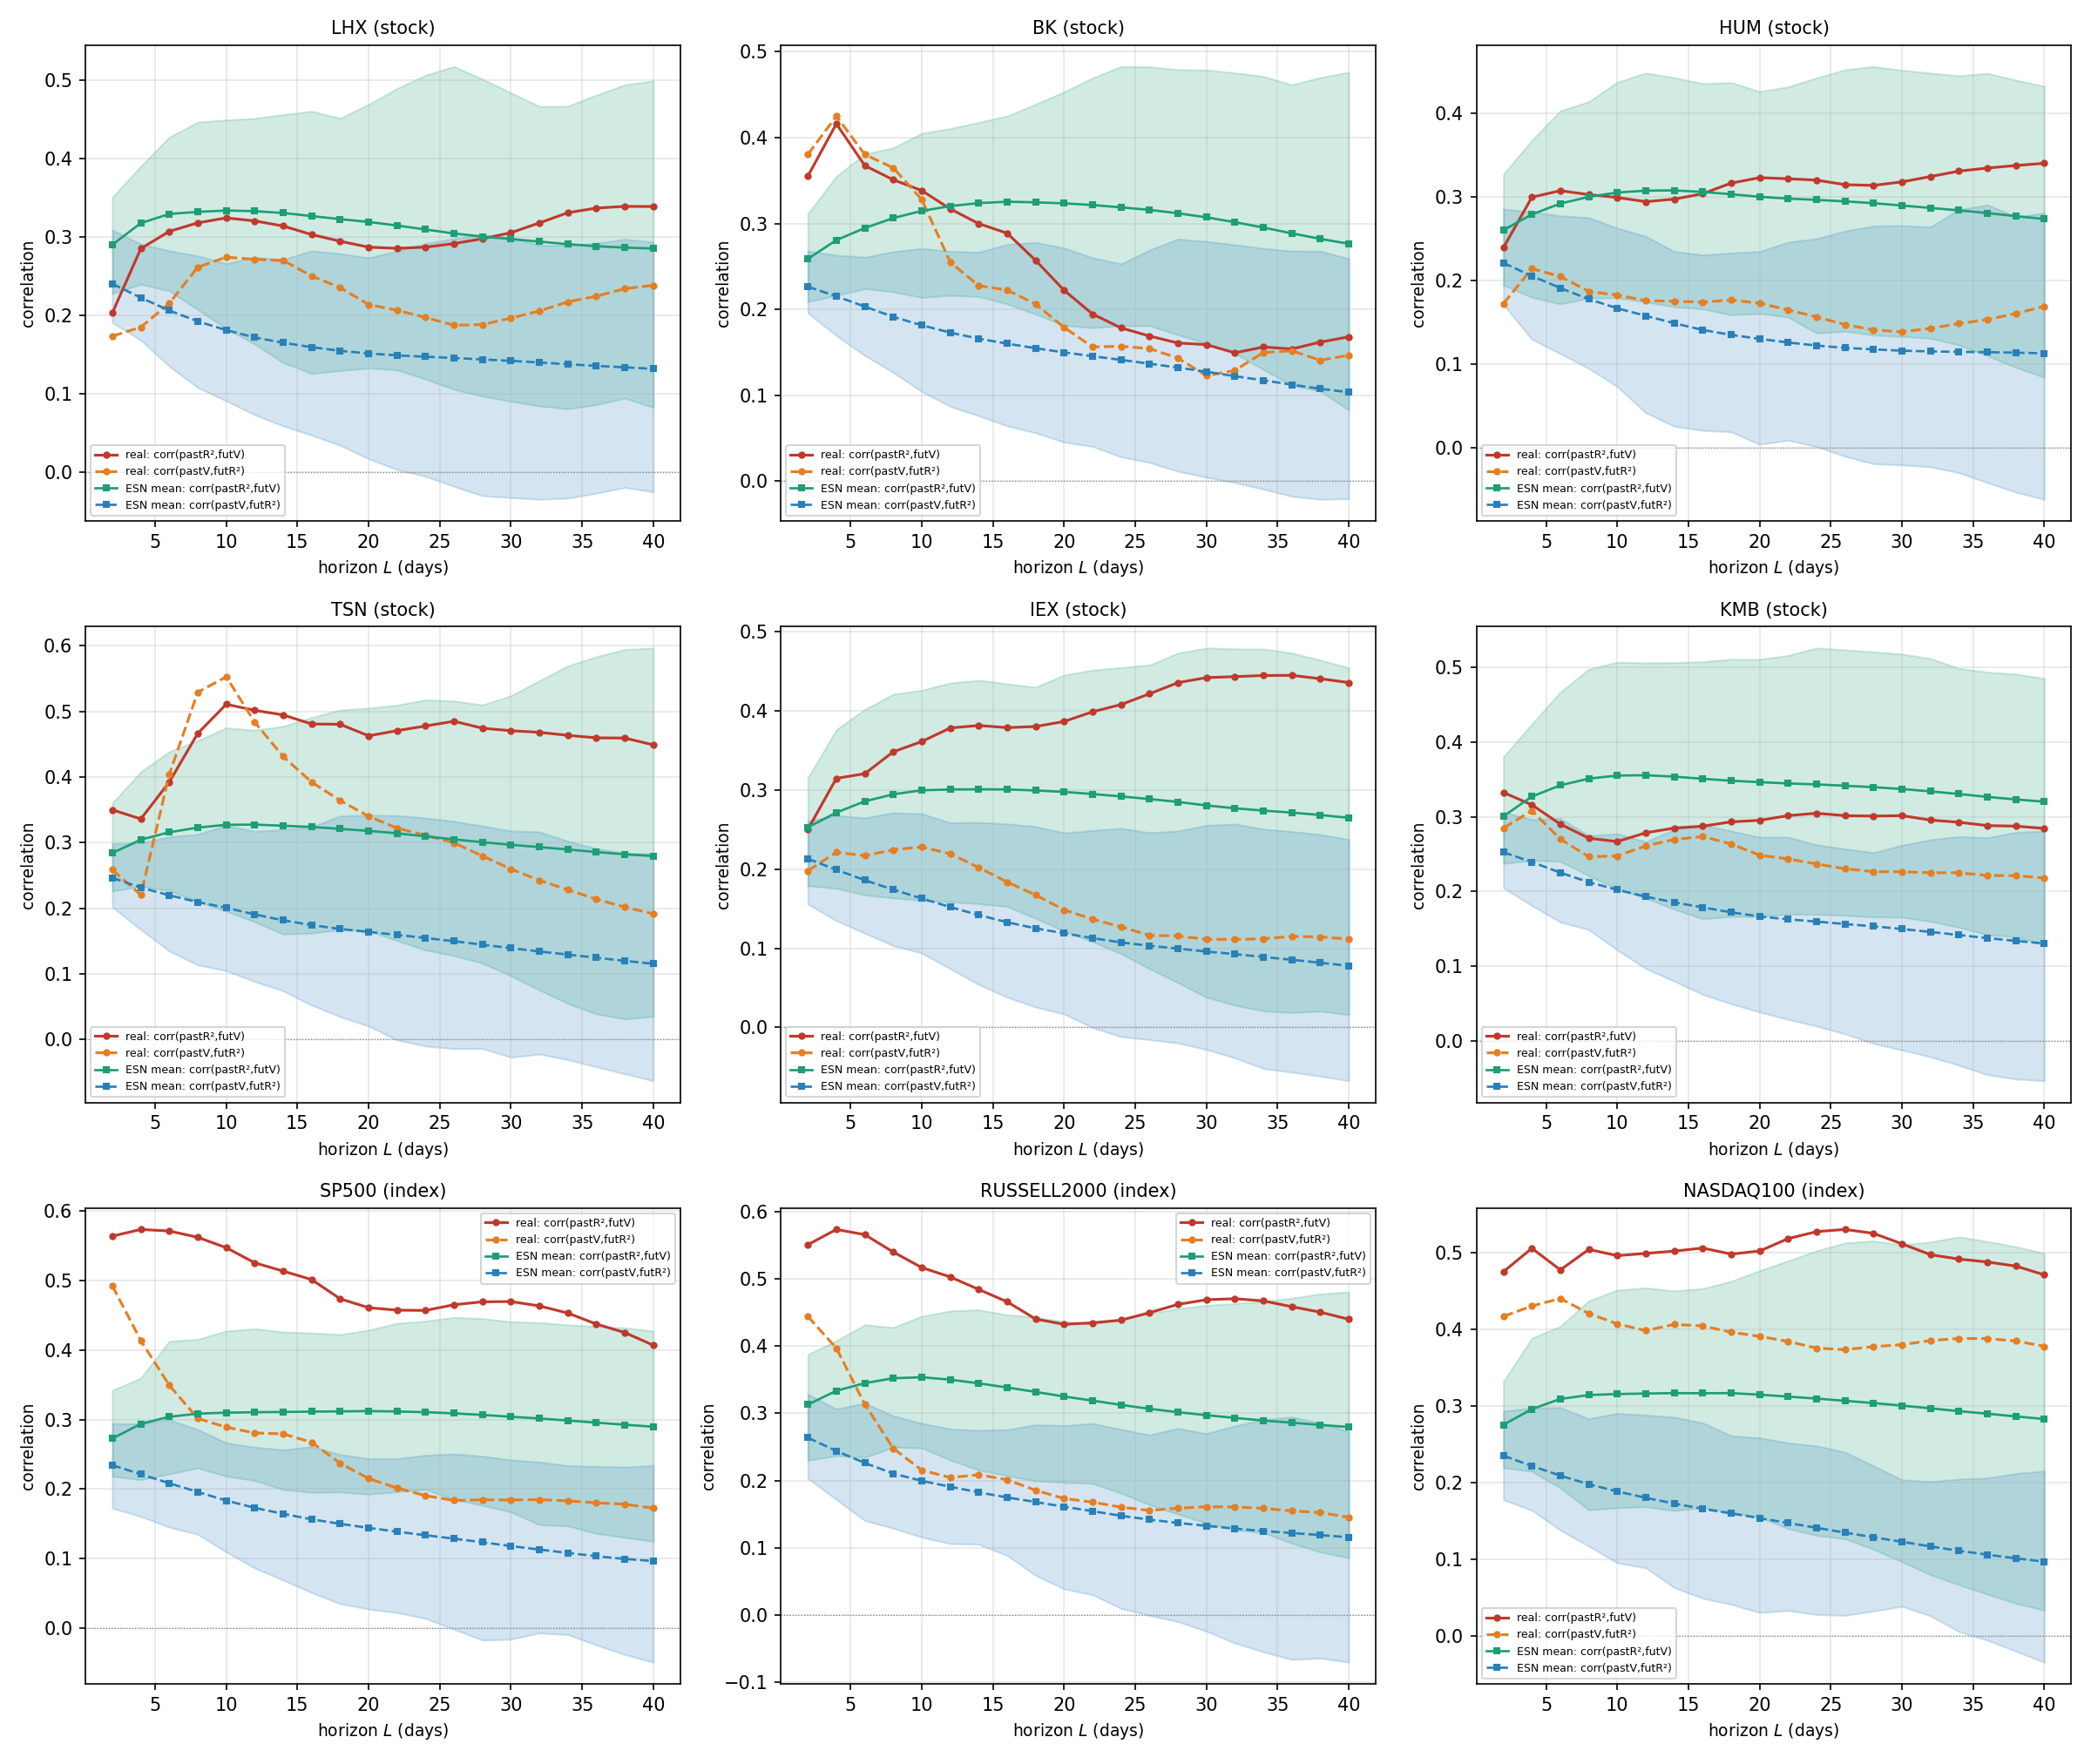
\includegraphics[width=0.98\textwidth]{zumbach_components_ci_bench9.png}
\caption{The 2 correlation components separately vs.\ horizon: real asset
(red/orange) vs.\ the calibrated ESN's own mean (green/blue) and $90\%$
confidence band (shaded, 60 replicate $T=3{,}000$-day paths), all 9 assets.}
\label{fig:zumbachcomponents}
\end{figure}

\begin{center}
\begin{tabular}{lccc}
\toprule
Asset & type & horizons inside $\text{Corr}(\text{past}R^2,\text{fut}V)$'s CI & horizons inside $\text{Corr}(\text{past}V,\text{fut}R^2)$'s CI \\
\midrule
\texttt{LHX}         & stock & $95\%$  & $90\%$  \\
\texttt{BK}          & stock & $70\%$  & $75\%$  \\
\texttt{HUM}         & stock & $100\%$ & $100\%$ \\
\texttt{TSN}         & stock & $80\%$  & $65\%$  \\
\texttt{IEX}         & stock & $100\%$ & $100\%$ \\
\texttt{KMB}         & stock & $100\%$ & $95\%$  \\
\texttt{SP500}       & index & $10\%$  & $60\%$  \\
\texttt{RUSSELL2000} & index & $30\%$  & $90\%$  \\
\texttt{NASDAQ100}   & index & $25\%$  & $0\%$   \\
\bottomrule
\end{tabular}
\end{center}

\textbf{For every one of the 6 stocks, both components individually match
real data about as well as their difference does} -- coverage stays at
$13$ or more of $20$ horizons for both components, consistent with
Figure~\ref{fig:zumbachwidened}'s own aggregate result. \textbf{For all 3
indices, the story is different}: $\text{Corr}(\text{past}R^2,\text{fut}V)$'s
own coverage collapses to $2$--$6$ of $20$ horizons, even though the same
3 indices showed good-to-excellent aggregate $Z(L)$ coverage in
\S\ref{sec:calibmethod}'s own results. Figure~\ref{fig:zumbachcomponents}
shows why: for all 3 indices, \emph{both} real components sit persistently
high (roughly $0.4$--$0.6$) while \emph{both} calibrated components sit
persistently lower (roughly $0.1$--$0.3$) -- the calibrated ESN undershoots
both correlations by a broadly similar amount, and \textbf{the aggregate
$Z(L)$ match for these 3 assets is, at least in part, 2 similarly-sized
errors cancelling in their difference, not 2 correlations each individually
reproduced.}

\section{Interpretation}
\textbf{The Zumbach effect's remaining gap was, like the leverage effect's
front-loading and the Taylor effect's persistence ceiling, a parameter bound
rather than a genuine architectural limit} -- and, as with the Taylor effect,
the limiting parameter was $\lambda_{hi}$'s own standard lower edge, not
$H$'s. This is now the second stylised fact in this note family where
$\lambda_{hi}=1.0$ specifically, used without individual scrutiny across
every calibration in this whole project, turns out to be too restrictive;
widening it and recalibrating resolves the gap with no other change to the
simulator or the architecture. \textbf{This resolution is real but partial
for the 3 indices specifically}: \S\ref{sec:components} shows their own good
aggregate $Z(L)$ coverage conceals a persistent, roughly $0.2$--$0.3$
undershoot in \emph{both} underlying correlations, not a genuine match at
the component level -- a caution directly analogous to the Taylor-effect
note's own finding that a single-scalar objective can look satisfied while
hiding a real shape mismatch underneath.

\section{Limitations and Recommended Next Steps}
\begin{enumerate}
\item \textbf{Every one of the 9 assets' own calibrated $H$ lands at or
within $0.045$ of its own standard upper bound, $0.3$}, and every
$\lambda_{lo}$ sits at its own lower bound, $10^{-5}$ -- both mirroring the
pattern that led to widening $\lambda_{hi}$ in the first place. Whether
either bound is also too narrow for the Zumbach effect specifically was not
tested here.
\item \textbf{\texttt{BK}, \texttt{TSN}, \texttt{KMB}, \texttt{SP500}, and
\texttt{RUSSELL2000} still fall short of full coverage} ($14$--$16$ of $20$
horizons). Whether this reflects a smaller residual gap still tied to a
further bound, or is closer to the edge of what a $90\%$ band from 60
replicates can be expected to cover even for a well-calibrated point, was
not investigated.
\item \textbf{$\lambda_{hi}$'s own new lower bound, $0.001$, was chosen
generously rather than tightly}: every asset's calibrated value falls
between $0.091$ and $0.145$, comfortably above this bound, but whether a
different asset bench might push closer to it was not examined.
\item \textbf{Whether widening $\lambda_{hi}$ disturbs any of the other 10
stylised facts calibrated elsewhere in this note family with $\lambda_{hi}$
held at its original, narrower range was not checked} -- a full re-run of
the companion note's own 5-asset, 11-stylised-fact calibration with this
bound widened would be needed to know whether this is a strict improvement
overall.
\item \textbf{The 3 indices' own persistent undershoot in both underlying
correlations (\S\ref{sec:components}) was not resolved.} Whether a further
bound-widening (e.g.\ on $H$ or $\lambda_{lo}$, both of which still sit at
their own bounds for every asset) would raise both components together, or
whether a genuinely different parameter is needed to separate them from
their difference $Z(L)$, was not tested.
\item \textbf{The 6 stocks and 3 indices were not chosen for any particular
economic or sectoral reason} -- the stocks are an independently randomised
selection (seed 2026), and the indices are the only 3 with available OHLC
data.
\end{enumerate}

\end{document}
